\subsection{RECOPILACIÓN DE BASES DE DATOS}

\subsubsection{Datos \emph{in-the-wild}}
Para evaluar las cadenas de procesamiento sobre conjuntos de datos de habla se emplea el corpus en español de Argentina recopilado por el grupo de investigación Intercambios Transorgánicos. Este corpus consta de 24 horas de grabaciones realizadas en condiciones heterogéneas —tanto en calidad de audio como en diversidad de hablantes— y proviene mayoritariamente de fuentes públicas en internet. Por su variabilidad y carácter no controlado, este conjunto \emph{in-the-wild} resulta idóneo para validar procedimientos de preprocesado de audio. En lo sucesivo, se hará referencia a esta colección como el conjunto de datos \emph{original} (versión sin procesamientos).

Con el objetivo de captar diferencias dialectales relevantes para Argentina, la selección de hablantes sigue la clasificación regional propuesta por \cite{Fontanella2004español}. En concreto, el corpus incluye 32 hablantes con acento bonaerense y 27 con acento centro, para un total de 59 hablantes. La estrategia a futuro consiste en ampliar la cobertura dialectal para incorporar todas las variedades representativas del país; sin embargo, en esta tesis se valida inicialmente la cadena de preprocesamiento sobre estas dos variantes representativas.

\subsubsection{Datos profesionales}
Para complementar el corpus \emph{in-the-wild} y disponer de material de mayor calidad contra el cual contrastar el análisis objetivo, se incorporan conjuntos de datos profesionales disponibles en trabajos previos. Dado que no existe una colección pública extensa exclusivamente de español de Argentina, se incluyen también recursos con variantes dialectales cercanas cuando procede.

\begin{itemize}
\item ELRA Dataset (\cite{google-arg}): aproximadamente 8 horas de audio con dialecto bonaerense, 44 hablantes.
\item Emilia (\cite{datset_arg}): aproximadamente 4 horas de audio (dialecto bonaerense). % Si se dispone del número de hablantes, añadir aquí.
\item HaCASpa Dataset (\cite{dataset_hamburg}): aproximadamente 10 horas de audio con dialecto bonaerense, 50 hablantes.
\end{itemize}

El conjunto profesional suma un total de 22 horas. 

\subsection{DESARROLLO DE LA CADENA DE PRE PROCESAMIENTO}

La cadena de preprocesamiento diseñada en esta Tesis es una secuencia modular y reproducible de etapas destinadas a transformar material \emph{in-the-wild} en subconjuntos utilizables para entrenamiento de TTS. Las etapas principales son las siguientes: 

\begin{enumerate}
\item Post-procesado y metadatos: Normalización de niveles, etiquetado de metadatos (origen, duración, dialecto, condiciones de captura) y generación de los subconjuntos finales para evaluación y para alimentación a modelos TTS.
\item Voice Activity Detection (VAD): Eliminación de segmentos sin voz y segmentación inicial en enunciados. En la implementación se usa Silero VAD (\cite{SileroVAD}) con una estrategia adaptativa de optimización de hiperparámetros basada en clasificar el ritmo de habla (lento/normal/rápido) mediante los timestamps de Whisper y optimizar los parámetros del VAD por categoría. Además, se controla la longitud final de las unidades (concatenación / recorte) para ajustarlas a la distribución requerida por modelos TTS downstream. 
\item Denoising / Speech enhancement: Aplicación opcional de la cadena para mitigar ruido y artefactos de grabación. Se evalúan modelos prácticos y eficientes en CPU, además de la opción sin denosing, considerando el balance entre mejora perceptual y preservación de la identidad vocal. Los modelos seleccionados son Demucs (\cite{demucs}) y DeepFilterNet (\cite{deepfilter}).
\item Filtrado de calidad no intrusivo: Evaluación y filtrado mediante modelos de calidad perceptual no intrusiva para aceptar o rechazar fragmentos según puntuación mínima. Se utiliza modelos predictivos de MOS (Mean-Opinion-Score) como métrica conjunta de calidad. Se evaluan los modelos NISQA (\cite{nisqa}) y DNS MOS (\cite{dns_mos}).
\item Transcripción (STT): Obtención de transcripciones automáticas necesario para obtener los pares texto-audio que se requieren para el entrenamiento; en esta etapa se prioriza la precisión a costa de un mayor tiempo de cómputo, dado el impacto de errores de transcripción en la calidad final del corpus. Se utiliza el modelo de Whisper Large para la transcripción (\cite{whisper}).
\end{enumerate}

La implementación enfatiza portabilidad y bajo costo computacional, de modo que grupos con recursos limitados puedan reproducir la cadena y comparar variantes de configuración sin necesidad de utilizar hardware de alto rendimiento como serían GPUs. El diagrama de flujo de toda  la cadena propuesta se presenta en la Figura \ref{fig:pipeline_flowchart}.

\begin{figure}[h]
  \centering
  \centerline{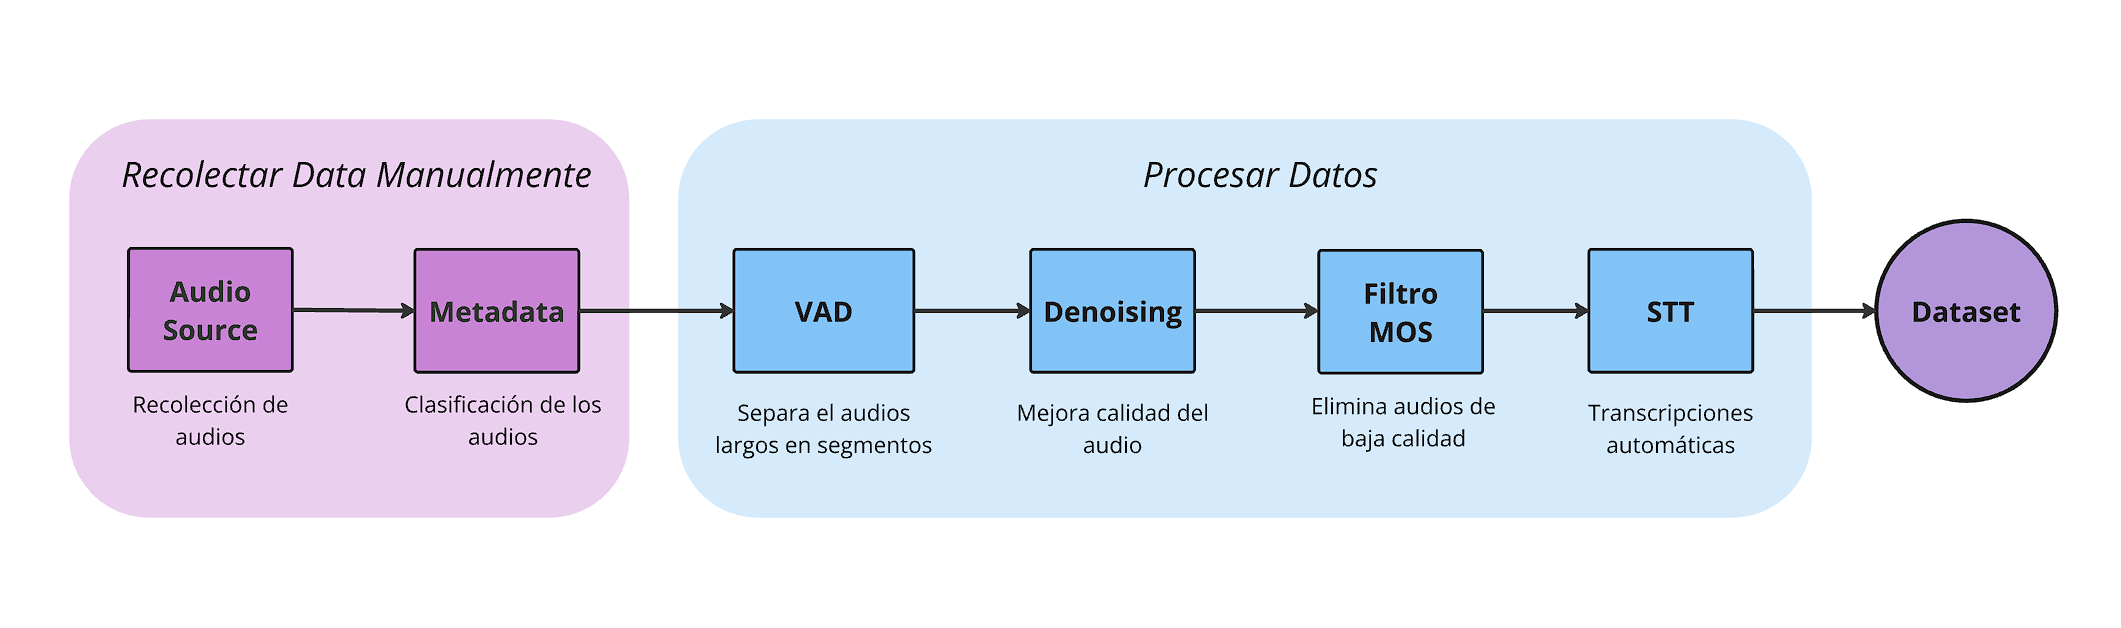
\includegraphics[width=18cm]{Figuras/Desarrollo/diagrama_flujo_cadena.PNG}}
  \caption{Diagrama de flujo del proceso completo para generar el dataset.}
    \label{fig:pipeline_flowchart}
\end{figure}

\subsubsection{Diferentes configuraciones}

Para evaluar el impacto de decisiones de diseño en la confección de cadenas de pre procesamiento, se proponen las siguientes variantes:

\begin{itemize}
    \item Condiciones de denoising: DeepFilterNet (DFN), Demucs, y \emph{no-denoising}. Estas alternativas representan puntos intermedios entre eficiencia, mejora perceptual y preservación de timbre. 
    \item Modelos de calidad no intrusiva: NISQA y DNSMOS, seleccionados por su uso extendido y su diferente sensibilidad a condiciones de ruido. Estos modelos son las mas usados en la literatura, donde se utiliza uno u el otro pero no se han contrastado para determinar el modelo mas optimo. 
    \item Umbrales de filtrado: Para NISQA se evaluaron (3.0, 3.5, 3.8, 4.2) y para DNSMOS (2.7, 3.0, 3.2, 3.4). Los umbrales se eligieron de forma empírica analizando el nivel predicho de MOS para todo el conjunto de datos original. 
\end{itemize}

La selección de umbrales parte de un análisis empírico presentado en la Figura \ref{fig:original_mos}, donde se calcula el valor de MOS resultante de NISQA y DNS MOS para todos los segmentos del dataset original. Es interesante notar como DNS MOS presenta un valor medio inferior y menos varianza. En consecuencia, para hacer una comparación justa, se seleccionaron los umbrales para garantizar un filtrado equitativo para los dos modelos.

\begin{figure}[h]
  \centering
  \centerline{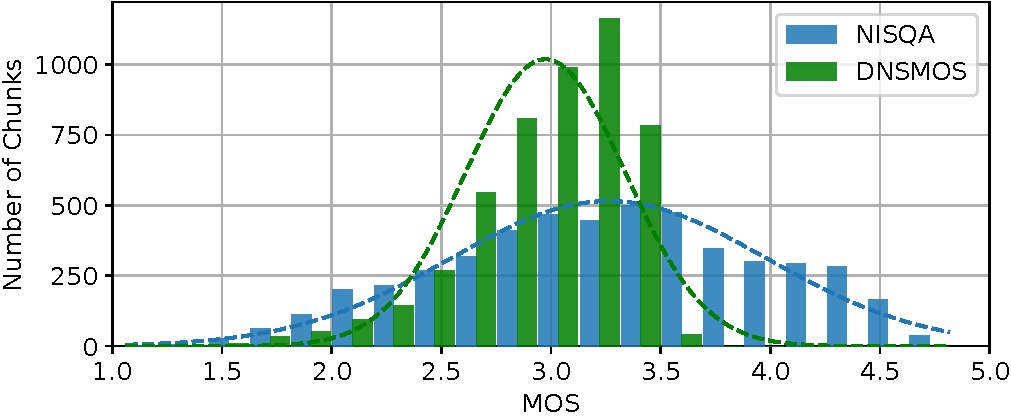
\includegraphics[width=13cm]{Figuras/Desarrollo/mos_pred_dist.pdf}}
  \caption{Resultado de MOS por cantidad de segmentos del dataset original para los 2 modelos a comparar.}
    \label{fig:original_mos}
\end{figure}

En la Figura \ref{fig:pipeline_variants} se presentan de manera gráfica las diferentes variantes a analizar. Cada configuración genera un subconjunto procesado sobre el que se calculan las métricas objetivas (ver sección siguiente) para permitir una comparación reproducible y dirigida por métrica sin necesidad de entrenar modelos TTS para cada variante. A estas variantes de procesamiento se las denomina sub dataset.

\begin{figure}[h]
  \centering
  \centerline{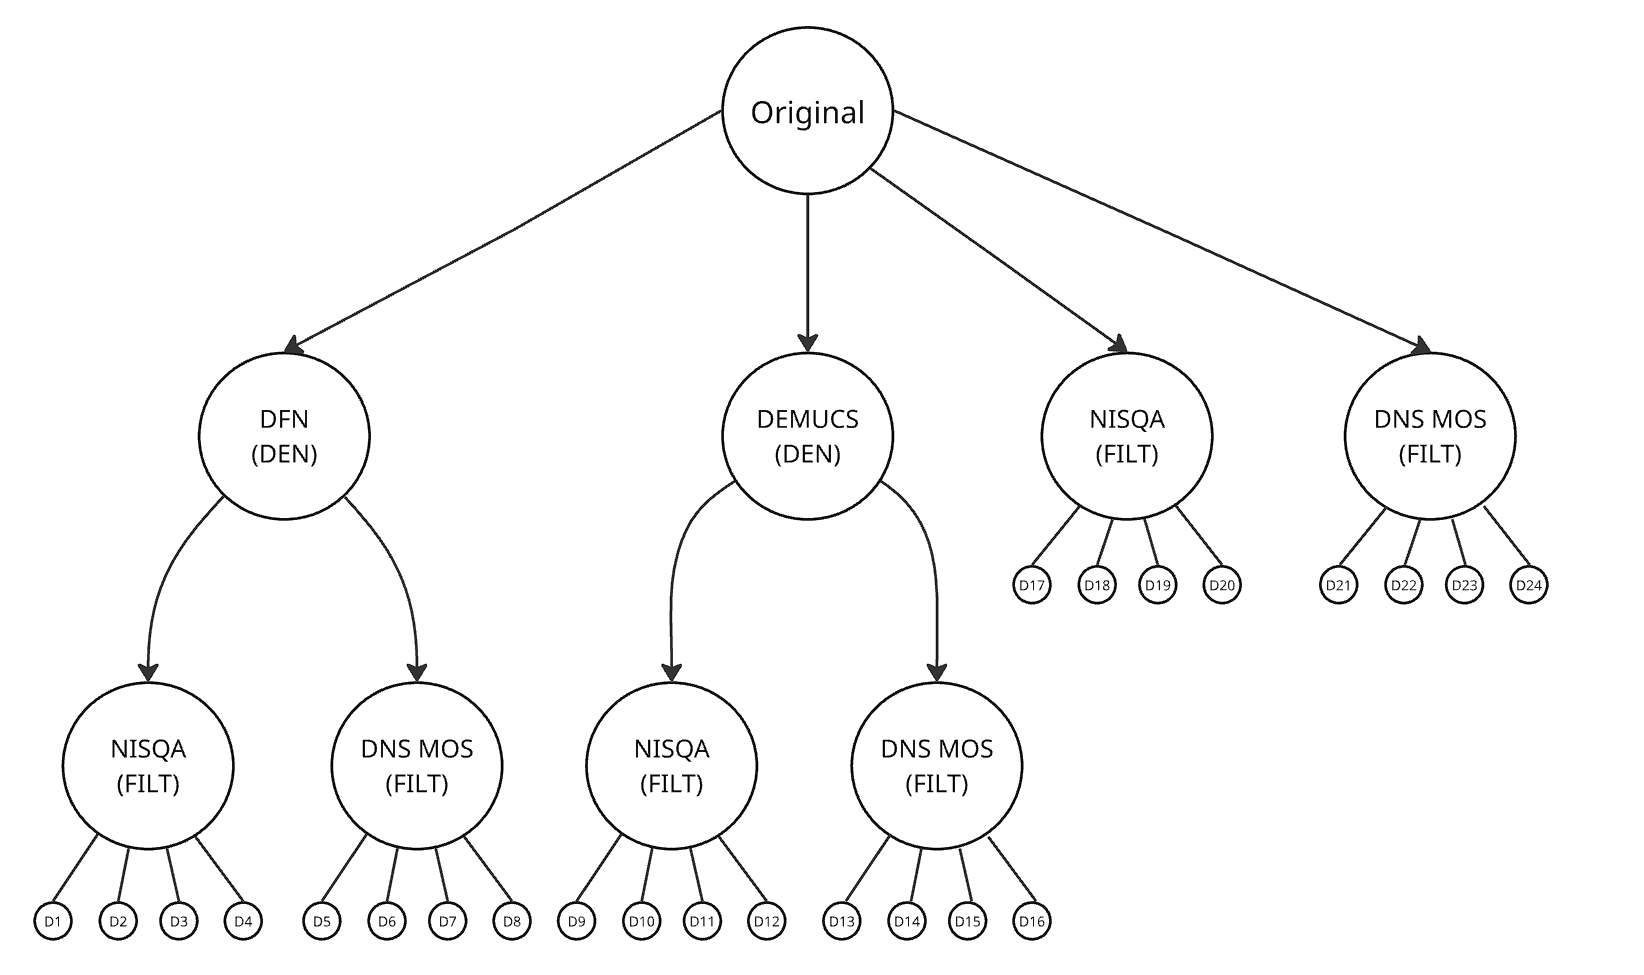
\includegraphics[width=15cm]{Figuras/Desarrollo/variantes_diagrama.PNG}}
  \caption{Variantes propuestas para evaluar diferentes configuración de la cadena de procesamientos.}
    \label{fig:pipeline_variants}
\end{figure}

\subsection{EVALUACIÓN DE LOS CONJUNTOS DE DATOS}
\label{sec:metricas_description}

La evaluación se articula alrededor de cuatro bloques de métricas complementarias que capturan cantidad, calidad de señal, condiciones acústicas y preservación de características del hablante. Estas métricas se combinan en una métrica compuesta que permite ordenar y seleccionar la mejor configuración según criterios definidos (ver formulación matemática al final). 

Todas las métricas buscan cuantificar diferencias relativas entre el dataset original y los sub datasets resultantes de las diferentes variantes; de esta forma, se pueden aplicar esta misma metodología de procesamiento para caracterizar el funcionamiento de la cadena de procesamientos, independientemente de las características del conjunto de datos de partida.

\subsubsection{Reducción del corpus}
El tamaño del dataset se mide en duración total (horas) y la \emph{reducción de datos} (RD) se cuantifica según Ecuación \ref{eq:horas}, donde el subíndice P hace referencia a las diferentes variantes del dataset procesado, y el subíndice O hace referencia a la cantidad de horas del dataset original.


\begin{equation}
\label{eq:horas}
RD_P = 1 - \frac{\mathrm{HORAS}_P}{\mathrm{HORAS}_O}
\end{equation}

Un valor de RD más pequeño es preferible (menos pérdida de datos). Esta medida captura el trade-off básico entre condiciones del filtrado agresivas y cantidad de material utilizable. 

\subsubsection{Calidad de la grabación}
La evaluación de la calidad de la grabación tiene por objetivo cuantificar, de forma objetiva y reproducible, las mejoras perceptuales y la fidelidad de la señal obtenidas tras aplicar las distintas etapas de la cadena (por ejemplo, denoising y filtrado). Para ello se emplean medidas complementarias: PESQ, SI-SDR y SNR; en un principio se contempla la posibilidad de utilizar también el STOI como un parámetro para cuantificar inteligibilidad, pero empíricamente no se encontraron diferencias significativas de este valor, con lo cual fue descartado. 

PESQ (Perceptual Evaluation of Speech Quality) se utiliza como un indicador aproximado de la calidad subjetiva de la señal comparando la versión procesada con la referencia original; SI-SDR (Scale-Invariant Signal-to-Distortion Ratio) mide la fidelidad de la señal de forma robusta frente a cambios de escala y permite evaluar cuánto contenido de la señal original se preserva tras el procesamiento; la definición teórica para calcular estos parámetros requiere de tener una versión original de la señal y una versión degradada, como en este caso se quiere comparar ambos dataset de forma independiente, se utiliza el modulo Pytorch Squim (\cite{squim}), que permite predecir los valores de PESQ, SI-SDR de forma no intrusiva (estimación ciega).

El SNR se estima mediante WADA-SNR (\cite{wada}) para obtener una cifra robusta de relación señal-ruido basada en la distribución de la amplitud de la onda. Todas estas métricas se computan a nivel de segmento y luego se resumen mediante la media y la desviación estándar para cada subconjunto, de modo que sea posible comparar distribuciones antes y después del procesamiento. Finalmente, las puntuaciones individuales se integran en el bloque \emph{Calidad señal} (CS) donde se suma la influencia de todos estos valores Ecuación \ref{eq:cs}, teniendo en cuenta que se espera que los valores de PESQ, SI-SDR y SNR suban (mejoría) al aplicar la cadena de procesamientos. Los subindices respetan la condiciones anterior donde P es por procesado y O es original, estos subíndices se mantiene consistentes para todas las métricas.

\begin{equation}
\label{eq:cs}
CS_P = 
\frac{\mathrm{PESQ}_O}{\mathrm{PESQ}_P}
\;+\; \frac{\mathrm{SI\text{-}SDR}_O}{\mathrm{SI\text{-}SDR}_P}
\;+\; \frac{\mathrm{SNR}_O}{\mathrm{SNR}_P}
\end{equation}

\subsubsection{Condiciones acústicas}
Las métricas acústicas buscan describir las condiciones de sala y la presencia de reverberación o de energía tardía en las grabaciones, aspectos que afectan la utilidad de los audios para entrenamiento de TTS, especialmente la alineación temporal entre texto y mel-spectrograma. En este trabajo se emplean descriptores clásicos como $T_{30}$ (tiempo de reverberación aproximado) y medidas de claridad como $C_{50}$ y $D_{50}$, que resumen la proporción de energía inicial frente a la energía reverberada y permiten detectar grabaciones con exceso de reverberación o mala claridad.

Nuevamente, es necesario calcular estos parámetros de forma ciega y sin referencia de las condiciones del entorno original,con estas limitaciones, estas métricas se estiman mediante un modelo CNN que fue entrenado para calcular parámetros acústicos de forma ciega, y fue validado para voces del español argentino, de manera que la estimación sea práctica sobre material \emph{in-the-wild} sin requerir respuestas impulsivas de sala (\cite{Maxi2}). Las mediciones se calculan por segmento y se agregan mediante estadísticos (media y desvío) para cada subconjunto; en la métrica compuesta se incorporan las mejores relativas para evaluar si una configuración reduce la reverberación y mejora la claridad respecto del conjunto original. 

En este caso, estas dos métricas se suman para contabilizar la influencia de las \emph{Condiciones acústicas} (CA) en la Ecuación \ref{eq:ca}, donde el $T_{30}$ mejora si disminuye, pero el $C_{50}$ mejora si se incrementa. Se descarta el $D_{50}$ ya que los resultados empíricos fueron muy similares al análisis del $C_{50}$, con lo cual no se estaría agregando información redundante y se decide en consecuencia eliminar el aporte de esta métrica. El análisis de estas variables permite discriminar configuraciones que mejoran la «condición de sala» del corpus sin sacrificar en exceso otros atributos.

\begin{equation}
\label{eq:ca}
CA_P = 
\frac{T_{30,P}}{T_{30,O}}
\;+\; \frac{C_{50,O}}{C_{50,P}}
\end{equation}

\subsubsection{Diferencias del habla}
Las medidas de diferencias del habla están pensadas para garantizar que las etapas de preprocesamiento, en particular los algoritmos de denoising, no alteren indebidamente la identidad del hablante ni la variabilidad prosódica del corpus, aspectos críticos para síntesis con preservación de timbre y estilo. En la tesis se consideran dos indicadores principales: la desviación estándar del F0 (F0-STD) y la distorsión mel-cepstral media (MCD). 

El F0-STD captura la variabilidad prosódica de los hablantes; su cálculo se realiza a nivel de segmento usando el estimador PESTO (\cite{PESTO}) para extracción robusta de pitch, y se compara entre versión original y procesada para detectar reducciones anómalas de variabilidad que indiquen pérdida de naturalidad o sesgo en la selección de hablantes. El MCD se calcula entre los coeficientes mel-cepstrales de la señal original y de la señal procesada (especialmente relevante en audios sometidos a denoising) para cuantificar cambios tímbricos (\cite{mcd_metric}); en la formulación adoptada el MCD se expresa como incremento porcentual o normalizada respecto a un valor de referencia aceptable de 5 dB según (\cite{survey2}), de esta forma se penalizan las configuraciones que alteran significativamente el timbre. 

Estas dos componentes se combinan en el bloque \emph{Diferencias del habla} (DH), donde cualquier diferencia relativa de F0-STD es penalizada, y lo mismo para el MCD respecto al valor de referencia Ecuación \ref{eq:dh}. Cabe aclarar que el MCD solo se calcula para las variantes con denoising, esto favorece de alguna forma a las variantes sin denoising que no modifican las características del hablante.

\begin{equation}
\label{eq:dh}
DH_P = 
\left|1 - \frac{\mathrm{F0std}_P}{\mathrm{F0std}_O}\right|
\;+\; \frac{MCD_P}{5}
\end{equation}

\subsubsection{Métrica conjunta}
Para ordenar configuraciones se propone una métrica compuesta que suma los cuatro bloques anteriores: reducción del dataset (RD), calidad de señal (CS), condiciones acústicos (CA) y diferencias de habla (DH). Esta métrica compuesta, plantea de forma matemática las relaciones de compromiso que se asumen con la cadena de procesamientos. 

Se plantea la métrica compuesta como un objetivo de optimización Ecuación \ref{eq:metric_total}, donde se busca minimizar el aporte negativo de cada variable para poder identificar la mejor variante P de la cadena de procesamientos.

\begin{equation}
\label{eq:metric_total}
\min_{P \in \mathrm{Conf}}\;
\Big\{
RD_{P}
\;+\;
CS_{P}
\;+\;
CA_{P}
\;+\;
DH_{P}
\Big\}
\end{equation}

Con esta formulación, configuraciones que mantienen mayor cantidad de horas, mejoran la calidad de señal, mejoran (o mantienen) condiciones acústicas y preservan características del hablante obtendrán puntuaciones más bajas (mejor). Se propone una configuración inicial donde todos los bloques tienen el mismo peso; la elección de pesos distintos permite priorizar, por ejemplo, la preservación vocal frente a la cantidad de horas si el objetivo es síntesis con alta fidelidad de identidad.

\subsection{ENTRENAMIENTO DEL MODELO DE ESTIMACIÓN DE DENSIDAD}
Explicar porque necesito hacer lo del modelo de estimación de densidad

\subsubsection{Validación con medelo zero-shot}
Definir modelo y explicar la justificación de este experimento

\subsection{DESCRIPCIÓN DE PRUEBAS ESTADÍSTICAS}
Detallar un poco las validaciones estadísticas que se van a realizar

\subsection{MODELO DE TTS ZERO-SHOT}
Definir el modelo de TTS a usar, el porque de la selección y la descripción del último experimento